\documentclass[12pt]{article}


\usepackage{braket}
\usepackage{amsmath}
\usepackage{amsfonts}
\usepackage{ulem}
\usepackage{graphicx}
\usepackage{float}
\usepackage{biblatex}
\usepackage{svg}
\usepackage[section]{placeins}

\graphicspath{{./img/}}
\addbibresource{Readings.bib}

%opening
\title{Quantum Kicked Rotor}
\author{Aditya Chincholi}

\begin{document}

\maketitle

\section{Introduction}

\section{Questions}
\begin{enumerate}
    \item What does kicking the rotor periodically have anything to do with
    a random walk?

    \item What is the analogy with Anderson localization? After all, Anderson
    localisation is about a diffusing wavefunction which encounters disorder in
    the form of passive scatterers and gets reflected/transmitted with certain
    probability. This transmission amplitude goes down exponentially with length
    of the sample. In contrast, in the kicked rotor we have an initial condition
    of uniform distribution in the position space. We have active ``kicks" which
    pump energy into the system and these kicks strengths are pseudo-random
    apparently.

    \item \label{ques:trulyrandom} If we take a quantum rotor and kick it with a
    truly random kick strength like $Ka_j$ at $t = j$ where $a_j = 1$ with
    probability $p$ and $a_j = -1$ with probability $1-p$, would it also show
    initial diffusion and subsequent localisation?

    \item In the Anderson localisation (at least for d=1 case), we see the
    ``transport" being matter transport i.e. we comment on the chances that the
    matter particle is transmitted across the sample. One could also say that
    the energy of the particle (which is constant) gets transported to position
    states far from the origin. But in the case of the kicked rotor, what
    exactly is being transported? Energy is being pumped into and taken out of
    this system at all levels, so what is being transported?

    \item \label{ques:timestepsbound} In the simulation, given a particular
    dimension of the fourier space of $\ket{\psi}$, how do we get a bound on
    the maximum timestep?

\end{enumerate}

\section{Partial Answers}
\begin{enumerate}
    \item Let us try and answer the question \ref{ques:trulyrandom}.
    First consider a hamiltonian given by:

    \begin{equation}
        H = \frac{L^2}{2} + \hbar K \sum_{j=0}^{\infty} a_j \delta(t - j)
    \end{equation}

    where $P(a_j = 1) = p, P(a_j = -1) = 1 - p$. We can take $p = \frac{1}{2}$
    for simplicity. We then have the unitary operator $U_j$ to evolve the state
    from after the (j-1)th kick to after the jth kick.

    \begin{align}
        U_j &= exp(-iKa_j) exp(-i\frac{L^2}{2\hbar}) \\
        U_j \ket{m} &= exp(-i (Ka_j + \frac{\hbar m^2}{2})) \ket{m}
    \end{align}
    where $\ket{m}$ is the eigenstate of angular momentum operator $L$.
    We can see clearly here that this random ``kick" actually does nothing.
    It doesn't project our system from one angular momentum eigenstate to
    another. So this is just a phase shift of each existing eigenstate.
    No new $\ket{m}$ states can be occupied which weren't occupied before.
    Clearly, the disorder $\leftrightarrow$ random kick strength analogy
    fails in this respect. Lets try the following general hamiltonian
    and find the problem.

    \begin{equation}
        H = \frac{L^2}{2}
            + \hbar K V(\theta) \sum_{j=0}^{\infty} a_j \delta(t - j)
    \end{equation}

    Then we get
    \begin{align}
        U_j &= exp(-iKa_jV(\theta)) exp(-i\frac{L^2}{2\hbar}) \\
        U_j \ket{m} &= 	\frac{e^{-i \hbar m^2/2}}{\sqrt{2\pi}}
        \int exp(-iKa_jV(\theta)) exp(-im\theta) \ket{\theta} d\theta \\
        &= 	\frac{e^{-i \hbar m^2/2}}{\sqrt{2\pi}}
        \int exp(-i(Ka_j\frac{V(\theta)}{\theta} + m)\theta) \ket{\theta} d\theta \\
        &[\text{And if we take } V(\theta) = \theta] = e^{-i \hbar m^2/2} \ket{m + Ka_j}
    \end{align}

    So clearly, $V(\theta)$ needs at least a $\theta$ term in order to kick the
    system into other states. The problem is that without theta dependence, the
    initial m term will never break into pieces which hop to other states.
    \sout{The issue is one cannot think of the state hopping from $\ket{m}$ to
    $\ket{n}$, rather one must look at it from the $\theta$ space perspective.}

    \item A naive answer to question \ref{ques:timestepsbound} might be to do
    the following energy calculation:
    \begin{align}
        T k &= \frac{1}{2} \hbar^2 L_{max}^2 \\
        T &\leq \frac{\hbar^2 L_{max}^2}{2 k} \\
        [\text{If we take } \hbar &= 1, L_{max} = 1000, k = 5] \nonumber \\
        T &\leq 10^5
    \end{align}
    which undoubtedly seems like an overestimate.
\end{enumerate}

\section{Week 7}
Deadline: Next Saturday (10 April 2021)
\subsection{Objectives}
\begin{enumerate}
    \item Work out the $a_j$ model analytically and computationally both.

    \item Add noise to kick period in the kicked rotor:
    Kick the rotor at $\tau \pm \delta\tau$ where $\delta\tau$ is drawn from a
    uniform distribution. Loss of localization is expected.

    \item Add noise to kick strength in the kicked rotor:
    Kick the rotor with strength $k \pm \delta k$ where $\delta k$ is from
    uniform distribution. Loss of localization is expected.

    \item Read up on the quasi-periodic kicked rotor and the metal-insulator
    transition in it.
\end{enumerate}

\section{Week 8}
Deadline: Saturday 17 April 2021 3:30 PM

\subsection{Problems with the results}
\begin{enumerate}
    \item In order to get the same results as them, we need to run till
    $t = 10^6$ steps, and for at least 1000 initial conditions of
    $(\phi_2, \phi_3)$. That comes to $10^9$ evolutions, which is a lot.
    And for $t = 10^6$, we'd have to account for diffusion in momentum space by
    taking as high a dimensionality for our simulation space. Time required for
    each time step goes over 2s per step for as low as 2001 dimensional space.
    For context, the run with 1000 timesteps, 201 dimensional space and 100
    initial conditions of $(\phi_2,\phi_3)$ took around 2 hrs.

    \item
\end{enumerate}

\section{Week 9}
\subsection{Driving Perturbation}
Consider the following Hamiltonian:

\begin{align}
    H &= \frac{p^2}{2}
    + K (1 + \epsilon cos(\omega_2 t + \phi_2) cos(\omega_3 t + \phi_3))
    \sum_{n \in \mathbb{Z}} \delta(t - n) + \lambda F_0 cos(\Omega t) \\
    &\text{Switching to the 3d rotor with quasimomenta.} \\
    H &= \frac{p_1^2}{2} + p_2 \omega_2 + p_3 \omega_3
    + K (1 + \epsilon \ cos\theta_2 \ cos\theta_3)
    \sum_{n \in \mathbb{Z}} \delta(t - n) + \lambda F_0 cos(\Omega t)
\end{align}

The time evolution from $n-1$ to $n-\Delta t$ is:

\begin{align}
    U_{\Delta t} &= exp(\frac{-i}{\hbar} \int_{n-1}^{n-\Delta t} dt H) \\
    &= exp(\frac{-i}{\hbar}\int_{n-1}^{n-\Delta t} dt (H_0 + \lambda H')) \\
    &= e^{-i (p_1^2/2 + p_2 \omega_2 + p_3 \omega_3)(1 - \Delta t) / \hbar} \
    e^{\frac{-i\lambda F_0}{\hbar \Omega}(sin(\Omega (n - \Delta t)) - sin(\Omega (n-1)))} \\
    F &= e^{-i k(1 + \epsilon cos\theta_2 cos\theta_3) / \hbar} \lim_{\Delta t \to 0} U_{\Delta t} \\
    F &= e^{-i k(1 + \epsilon cos(\omega_2 n + \phi_2) cos(\omega_3 n + \phi_3)) / \hbar} \ e^{-ip^2/2\hbar} \  e^{-i\lambda F_0(sin(n \Omega) - sin((n-1) \Omega )) / \hbar \Omega}
\end{align}

\sout{This is under the approximation that the hamiltonian $H$ is
dominated by the kick term during the interval $n-\Delta t$ to $n$.
That implies that $|cos(n\Omega)\Delta t| << k (1 - \epsilon)$ where
$\Delta t$ is the width of the kick pulse in a physical setting.}


\section{Week 10}
\subsection{Goals}
\begin{itemize}
    \item To find out a way to calculate the bipartite entanglement between the
    $\ket{p_1}$ states and the $\ket{p_2, p_3}$ states in the quasiperiodic
    kicked rotor.

    \item To better express the phase driving perturbation from last time.

    \item To try out the driving term as a perturbation to the kicked rotor.
\end{itemize}

\subsection{Bipartite Entanglement Calculation}
\begin{itemize}
    \item First of all, we want to stick to simulating the 1d quasiperiodic
    kicked rotor. In order to simulate the 3d form, our floquet operator would
    require $O(N^6)$ entries where N is the size of the momentum spaces along
    each angle. This is not feasible for accuracy in a simulation. There is a
    possibility, however, that we use sparse matrices and reduce the size of
    the stored operator as it need only be calculated once but the density
    operator will also be of the same size and that is not sparse.

    \item The first issue I tried to tackle was to find a good way to represent
    the $F_{3d}$ operator. However, that involved a fourier transform of the
    following which I have no clue how to solve. The 1d case came from an vague
    Bessel function relation which I couldn't really apply here. In any case,
    the $\theta's$ would definitely get mixed up in the final result as
    entanglement is happening so there's no straightforward way to do this:
    \begin{equation}
        \frac{1}{(2\pi)^3} \int d^3\theta \
        e^{-i k cos(\theta_1)[1 + \epsilon cos(\theta_2)  cos(\theta_3)] / \hbar}
        e^{-i (\bf{m - n}) \cdot \boldsymbol{\theta}}
    \end{equation}

    So I resorted to numerically evaluating it. It took a while to understand the
    discrete fourier transform code, but I wrote it.

    \item The main theoretical considerations I tried was trying to get a
    relation between the 1d rotor and the 3d rotor. But despite trying to
    manipulate the kets for a long time, I couldn't really do much. I tried
    taking the trace of $F_{3d}$ and that did yield a relation to $F_{1d}$ but
    the bipartite entanglement requires $\rho_1 = tr_{2,3}(\rho)$ which cannot
    be reduced to just the trace of $F_{3d}$.

    \begin{equation}
        tr_{2,3}(F_{3d}) = \sum_{m_1, n_1} \sum_{m_2, m_3}
        \ket{m_1}\bra{n_1} e^{-i(m_2\omega_2 + m_3\omega_3)}
        \int \int \frac{d\theta_2 d\theta_3}{(2\pi)^2} (F_{1d})_{nm})
    \end{equation}

    \item Last night's work:
    \begin{equation}
        \mathbb{P}_{\varphi_2+\omega_2,\varphi_3+\omega_3}
        F_{3d} \mathbb{P}_{\varphi_2,\varphi_3} = F_{1d}
        \otimes \mathbb{I} \otimes \mathbb{I}
    \end{equation}
\end{itemize}

\section{Week 11}
\subsection{Goals}
\begin{itemize}
    \item Program and calculate the bipartite entanglement
    by simulating the 3d kicked rotor.

    \item Read and understand the paper on ``Multifractility ..."
    and compare with my results.

    \item Read and work out the critical point dynamics from
    Muller, Delande's paper.
\end{itemize}

\subsection{Floquet Expression Derivation}

\begin{align*}
    F_{3d} &= e^{-i K cos\theta_1 (1 + \alpha cos\theta_2 cos\theta_3) / \hbar}
    e^{-i (p_1^2 / 2 + p_2 \omega_2 + p_3 \omega_3)/\hbar} \\
    \bra{\mathbf{m}} F_{3d} \ket{\mathbf{n}} &=
    \bra{m_1, m_2, m_3}F_{3d}\ket{n_1, n_2, n_3} \\
    &= \bra{\mathbf{m}}
    e^{-i K cos\theta_1 (1 + \alpha cos\theta_2 cos\theta_3) / \hbar}
    \ket{\mathbf{n}} e^{-i (\hbar n_1^2 / 2 + n_2 \omega_2 + n_3 \omega_3)} \\
    &= \bra{\mathbf{m}} \int_{[0,2\pi]^3} d^3\theta \
    e^{-i K cos\theta_1 (1 + \alpha cos\theta_2 cos\theta_3) / \hbar}
    \ket{\boldsymbol{\theta}}\braket{\boldsymbol{\theta}|\mathbf{n}}
    e^{-i (\hbar n_1^2 / 2 + n_2 \omega_2 + n_3 \omega_3)} \\
    &= \int_{[0,2\pi]^3} d^3\theta \ \braket{\mathbf{m}|\boldsymbol{\theta}}
    e^{-i K cos\theta_1 (1 + \alpha cos\theta_2 cos\theta_3) / \hbar}
    \braket{\boldsymbol{\theta}|\mathbf{n}}
    e^{-i (\hbar n_1^2 / 2 + n_2 \omega_2 + n_3 \omega_3)} \\
    &= e^{-i (\hbar n_1^2 / 2 + n_2 \omega_2 + n_3 \omega_3)}
    \frac{1}{(2\pi)^3} \int_{[0,2\pi]^3} d^3\theta \
    e^{-i(\mathbf{m} - \mathbf{n})\cdot \boldsymbol{\theta}}
    e^{-i K cos\theta_1 (1 + \alpha cos\theta_2 cos\theta_3) / \hbar}\\
    &\approx e^{-i (\hbar n_1^2 / 2 + n_2 \omega_2 + n_3 \omega_3)}
    DFT_N(f(\boldsymbol{\theta}))[\mathbf{m} - \mathbf{n}]\\
    \text{where }
    f(\boldsymbol{\theta}) &=
    e^{-i K cos\theta_1 (1 + \alpha cos\theta_2 cos\theta_3) / \hbar}
\end{align*}

\newpage

\section{Bipartite Entanglement Simulation}
\subsection{Results}

\begin{figure}[h]
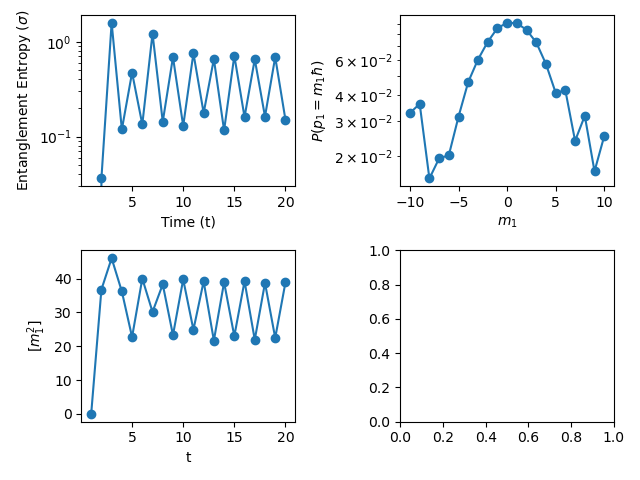
\includegraphics[width=\linewidth]{entanglement_entropy}
\centering
\end{figure}

\begin{enumerate}
    \item Bipartite entanglement entropy between the two subspaces
    $\mathcal{H}_1$ and $\mathcal{H}_{2,3}$ is non-zero and is roughly
    $O(10^{-1})$. It seems to saturate or at least oscillate about a
    mean. But there are issues.

    \item The momentum $p_1$ distribution looks sort of correct. But it
    is clear that we need more basis states based on the rise at the
    edges of the distribution.

    \item The momentum square $p_1^2$ is increasing properly like a
    diffusive regime and then saturating out due to lack of basis states.
\end{enumerate}

\subsection{Issues}

\begin{figure}[h]
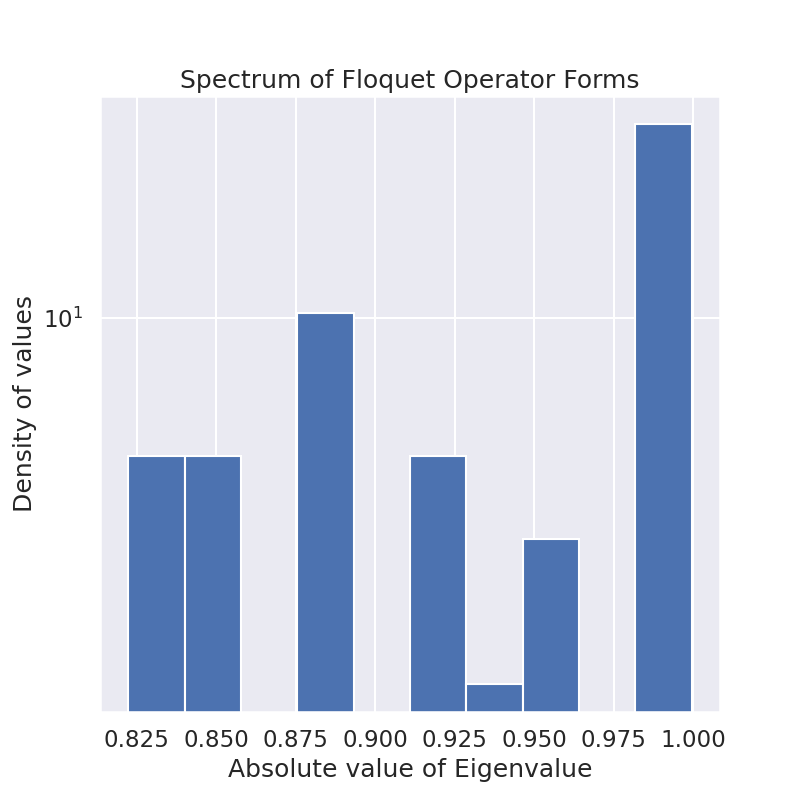
\includegraphics[width=\linewidth]{floquet_spectrum_21}
\centering
\caption{This plot was made from 1331 eigenvalues. Also it should be
number of values not density.}
\end{figure}

\begin{figure}[h]
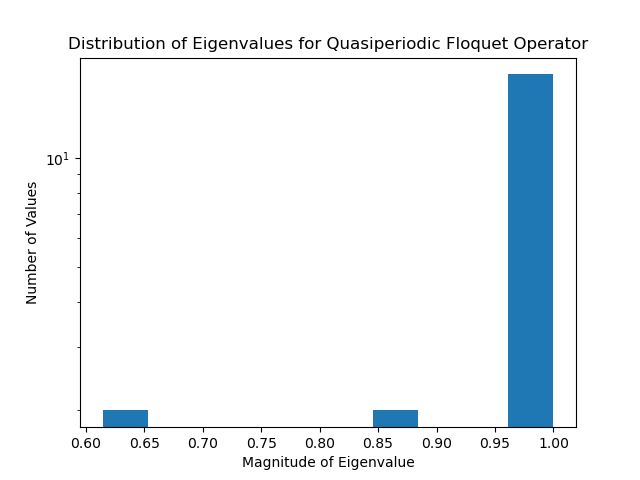
\includegraphics[width=\linewidth]{quasiperiodic_floquet_eigenval_dist_10}
\centering
\end{figure}

\begin{enumerate}
    \item First of all, the matrix is not unitary. It's eigenvalue
    spectrum is not composed of phases. For a $21^3 \times 21^3$
    case, 1331 eigenvalues were calculated for the matrix and they
    had a decent amount of spread. Calculating the determinant,
    through logdet, also yields very small quantities $e^{-O(100)}$.

    But this is just with the dense form of the matrix. In order
    to decrease memory consumption, we use sparse matrices. So we zero
    out any terms with absolute value less than $10^{-6}$. Should be a
    reasonable thing to do. Apparently not, because the eigenvalues
    amplitudes shot up to 10-12 when I tried finding eigenvalues of the
    sparse matrix. But I could not repeat this computation.
    Every time I tried again, ARPACK (used by scipy) said all the
    eigenvectors failed to converge.

    It is notable that this is happening despite various tests
    telling me that the floquet operator expression is correct. I have
    run tests wherein one of the elements is computed through quad instead
    of the fft and it matches it to a good degree.

    \item The other issue, due to the first one, is that the trace of the
    density matrix is not conserved to be unity. For lower dimensions, the
    difference is very small, it goes from 0.99 to 0.97 to 0.89 to 0.6.
    In this case, one can possibly justify a simple correction to divide
    $\rho$ by the $tr(\rho)$ or by $tr(\rho_1)$. But this is harder for
    higher dimensions because the fluctuations tend to increase. I have to
    correct by dividing by $tr(\rho)$ here, $tr(\rho_1)$ also fails here.

    \item The calculation of the floquet matrix has been parallelized,
    and it's sparse form takes relatively low amount of space in memory.
    But the density matrices are, well, dense. They cannot be sparse.
    So the evolution takes place with a Sparse $\times$ Dense $\times$
    Sparse dot product operation. But sparse linalg is single-threaded.
    And that's the case in pretty much all libraries available across
    major languages (MATLAB included). So the evolution is slow. And
    by slow I mean quite slow. It took over an hour to do 20 timesteps
    in the 21 basis case.

    \item I cannot afford to use dense forms of the floquet operator on my
    system. The system already uses 3.7 GB of RAM and ~2 GB of swap
    space on my system with 21 basis states for each subspace. When
    I tried increasing this to 24 basis states per subspace, the
    program segfaulted. So having a dense floquet operator is not an
    option on my system at least.

    I have also tried using a smaller datatype (complex32 over complex64),
    but that started giving me underflow errors and NaNs. I tried mitigating
    them, but eventually I had to move to the larger datatype as the processing
    became very problematic.
\end{enumerate}

\section{Spectral Analysis}

\begin{figure}[h]
    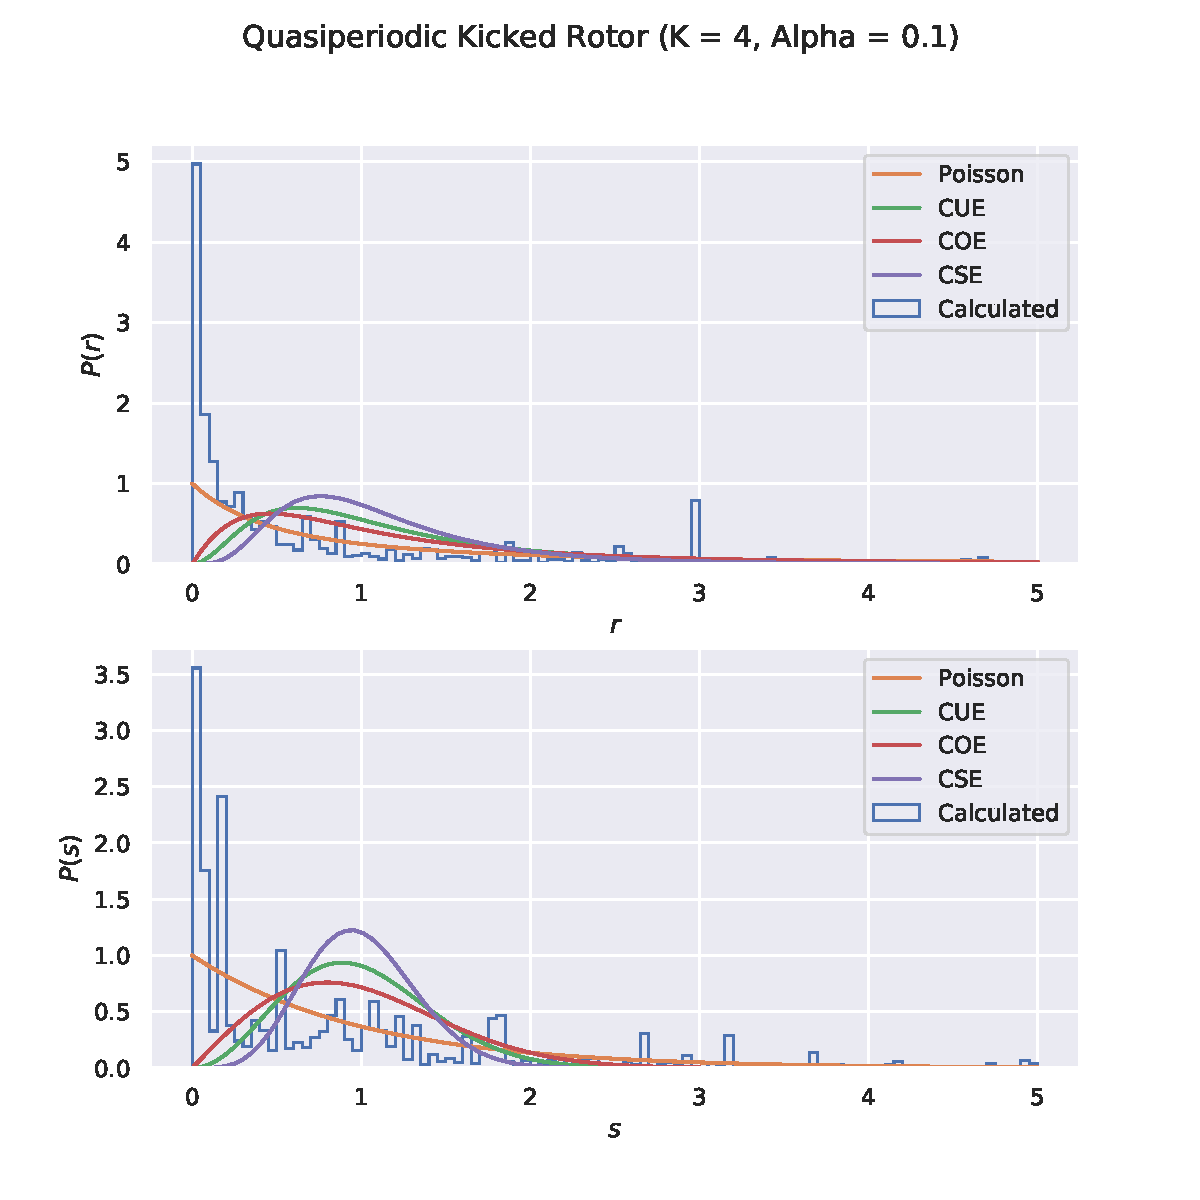
\includegraphics[width=\linewidth]{quasiperiodic_kickedrotor_spectrum_N10_precritical.pdf}
    \caption{Precritical: $p$ in (-10, 10), K = 4, $\hbar$ = 2.85, $\alpha$ = 0.1,
    $\omega_2$ = $2\pi\sqrt{5}$, $\omega_3$ = $2\pi\sqrt{13}$, eigenphases
    used = 8379 and 882 were discarded due to magnitude errors. $det(F) = 9.7
    \times 10^{-96} - i 3 \times 10^{-96}$.}
    \centering
\end{figure}

\begin{figure}[h]
    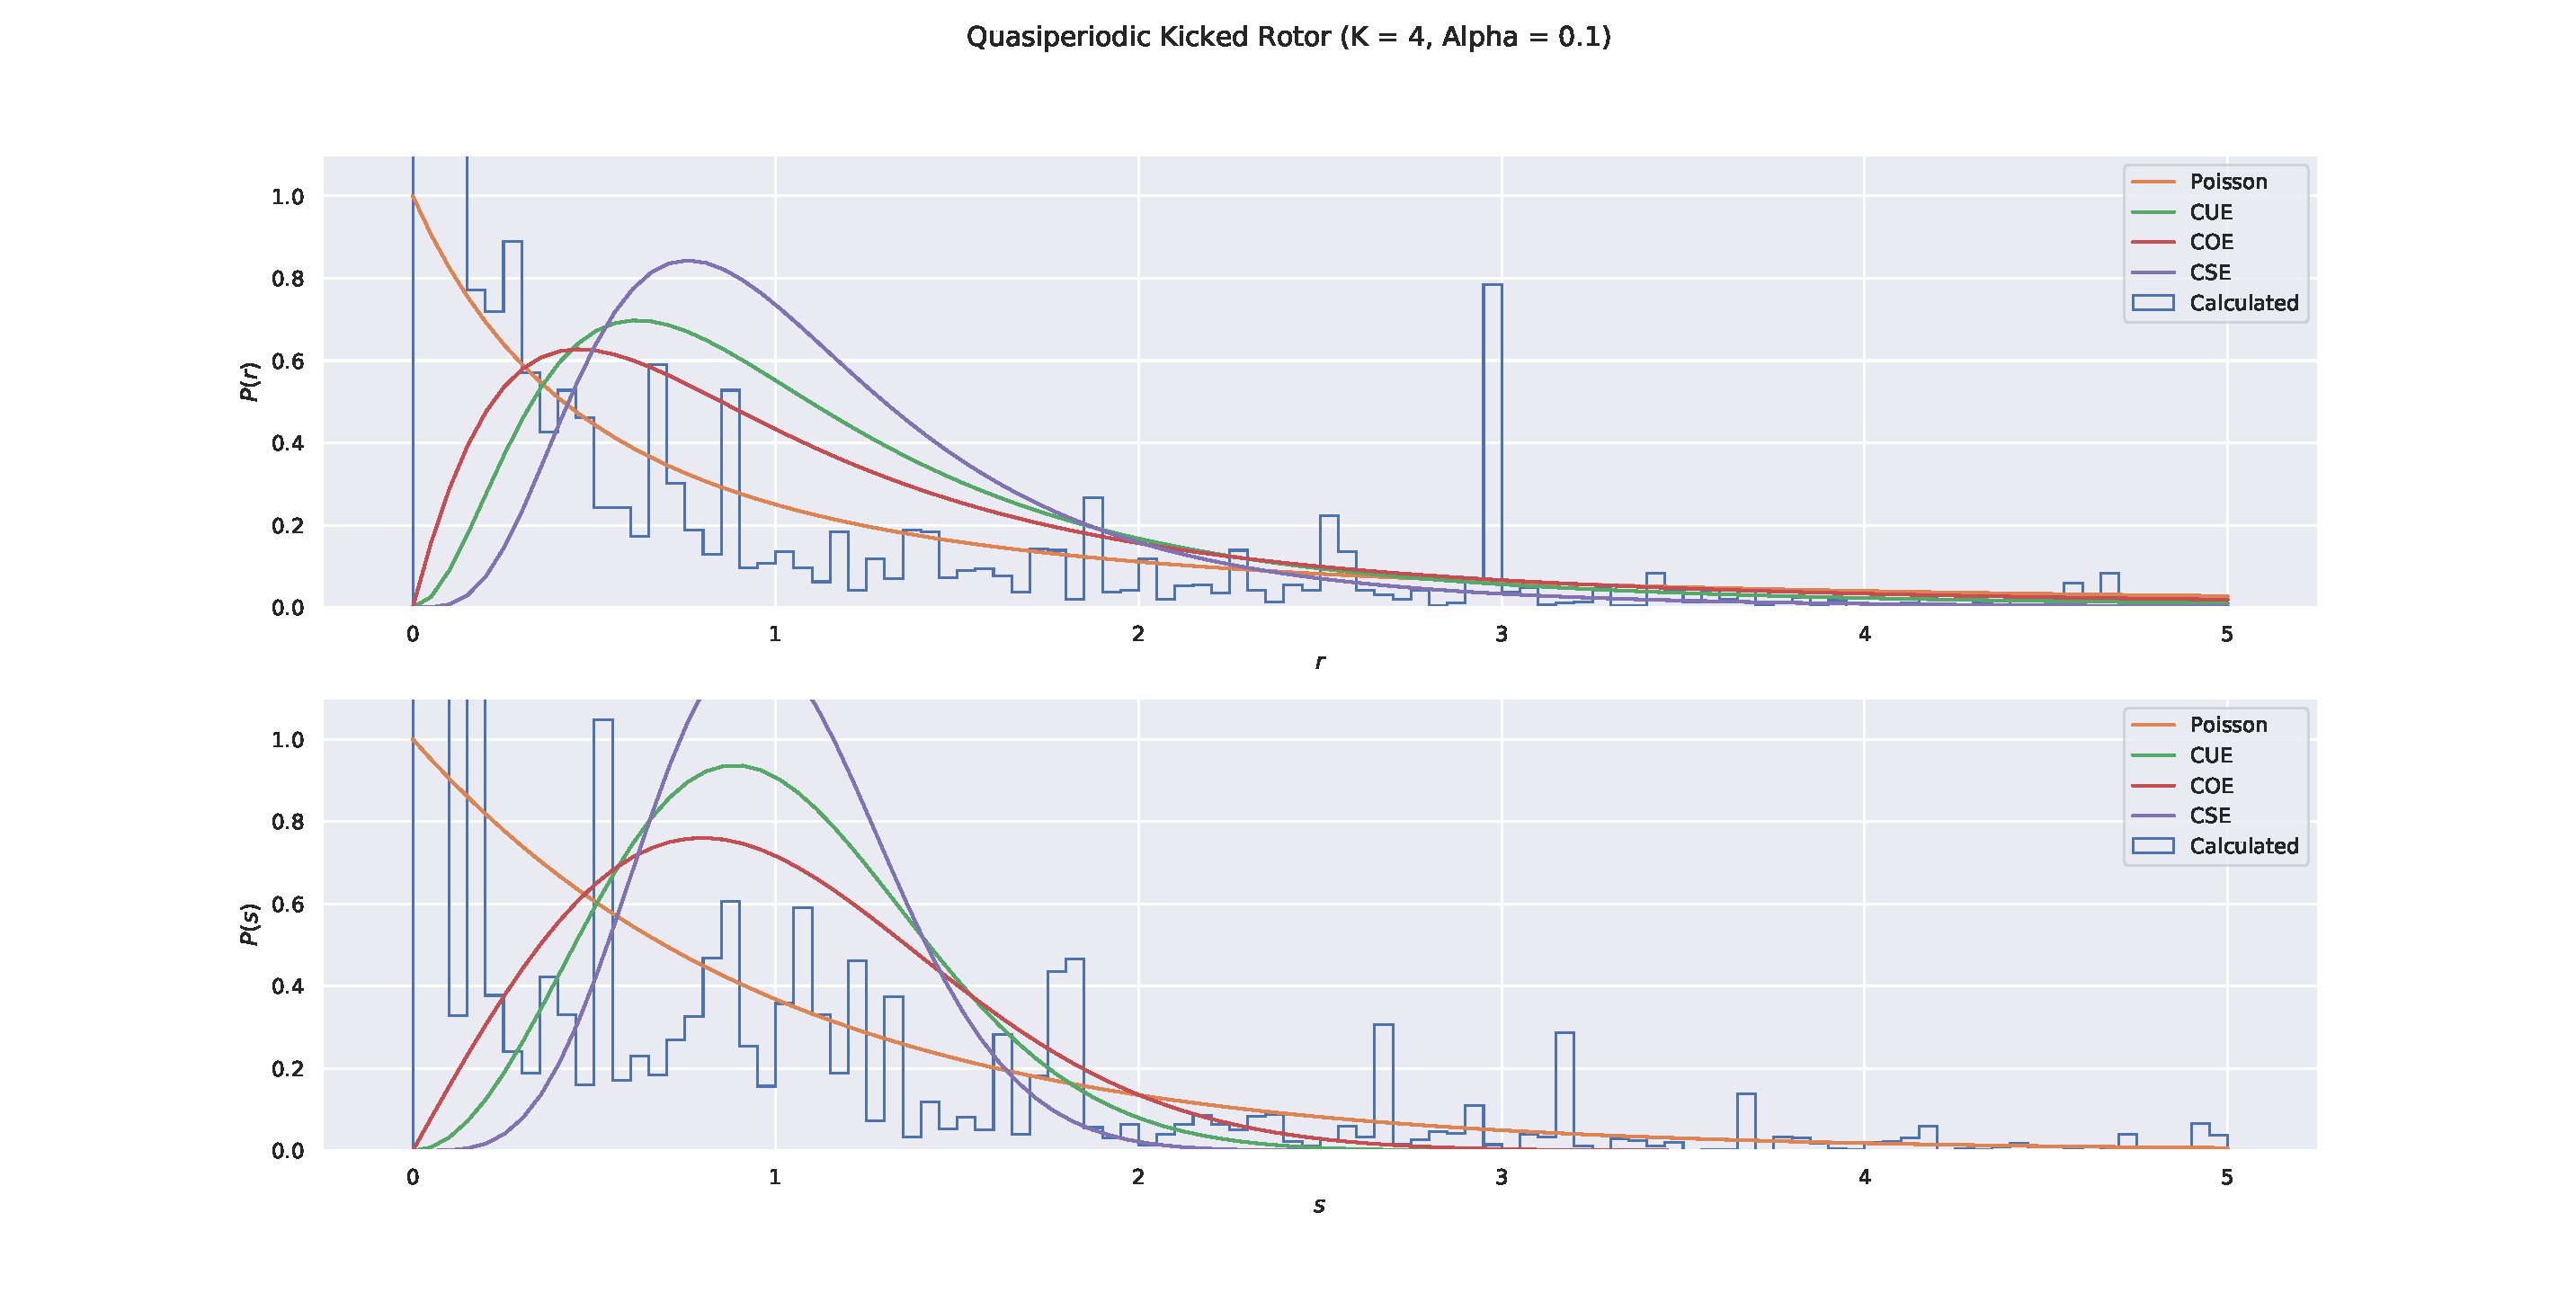
\includegraphics[width=\linewidth]{quasiperiodic_kickedrotor_spectrum_N10_precritical_magnified.pdf}
    \caption{Same as last one just magnified.
    Precritical: $p$ in (-10, 10), K = 4, $\hbar$ = 2.85, $\alpha$ = 0.1,
    $\omega_2$ = $2\pi\sqrt{5}$, $\omega_3$ = $2\pi\sqrt{13}$, eigenphases
    used = 8379 and 882 were discarded due to magnitude errors. $det(F) = 9.7
    \times 10^{-96} - i 3 \times 10^{-96}$.}
    \centering
\end{figure}

\begin{figure}[h]
    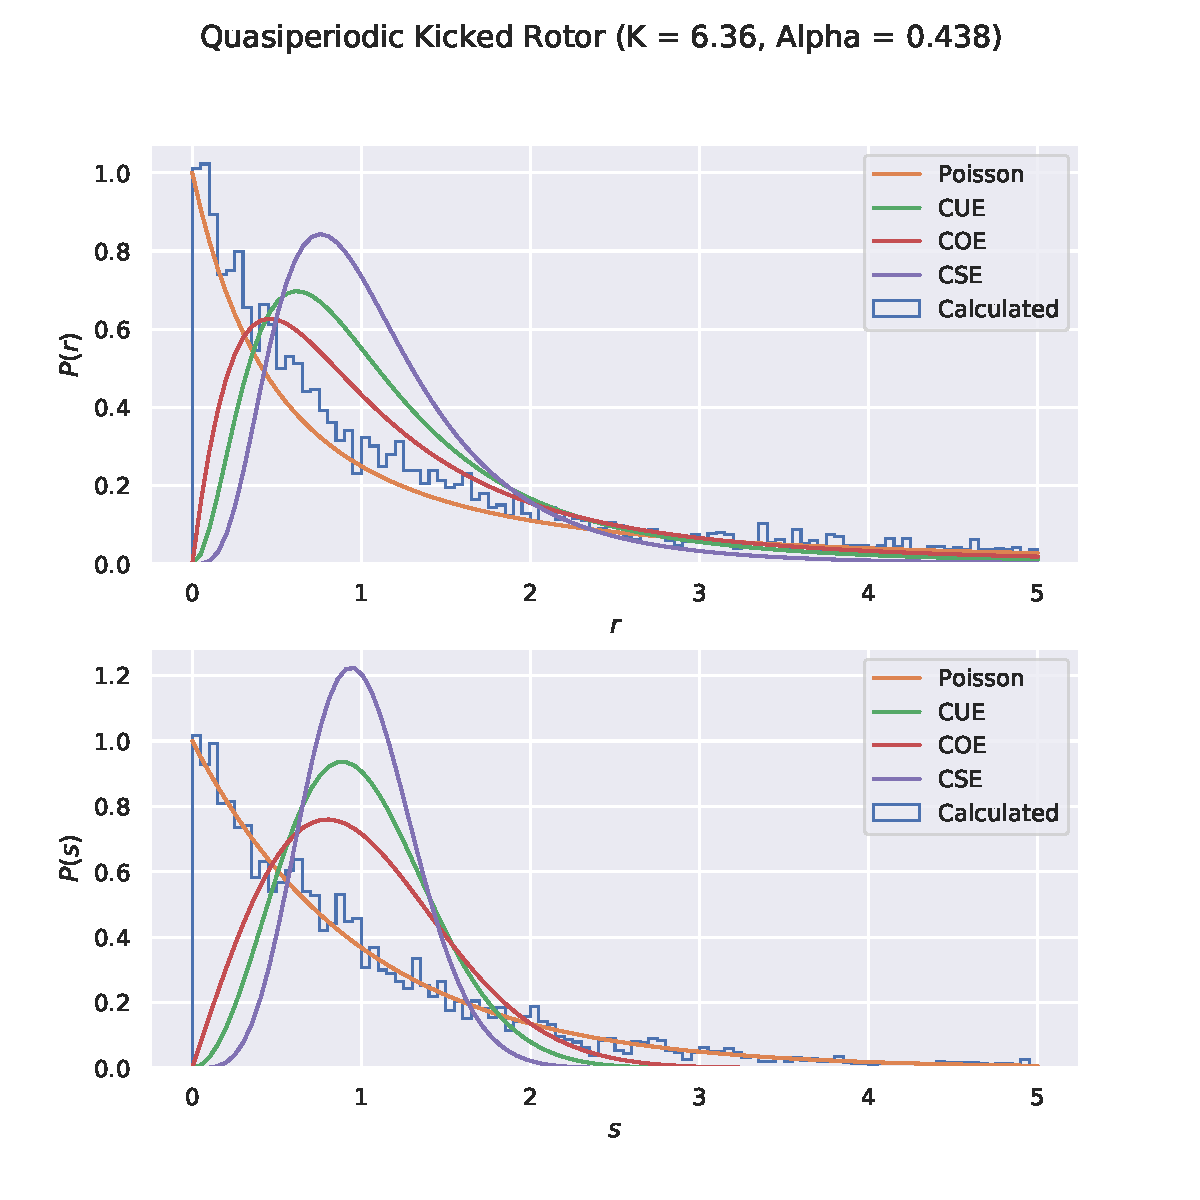
\includegraphics[width=\linewidth]{quasiperiodic_kickedrotor_spectrum_N10_critical.pdf}
    \caption{Critical: $p$ in (-10, 10), K = 6.36, $\hbar$ = 2.85, $\alpha$ = 0.438,
    $\omega_2$ = $2\pi\sqrt{5}$, $\omega_3$ = $2\pi\sqrt{13}$, eigenphases
    used = 7874 and 1387 were discarded due to magnitude errors. $det(F) =
    6.335 \times 10^{-272} - i 1.959 \times 10^{-272}$.}
    \centering
\end{figure}

\begin{figure}[h]
    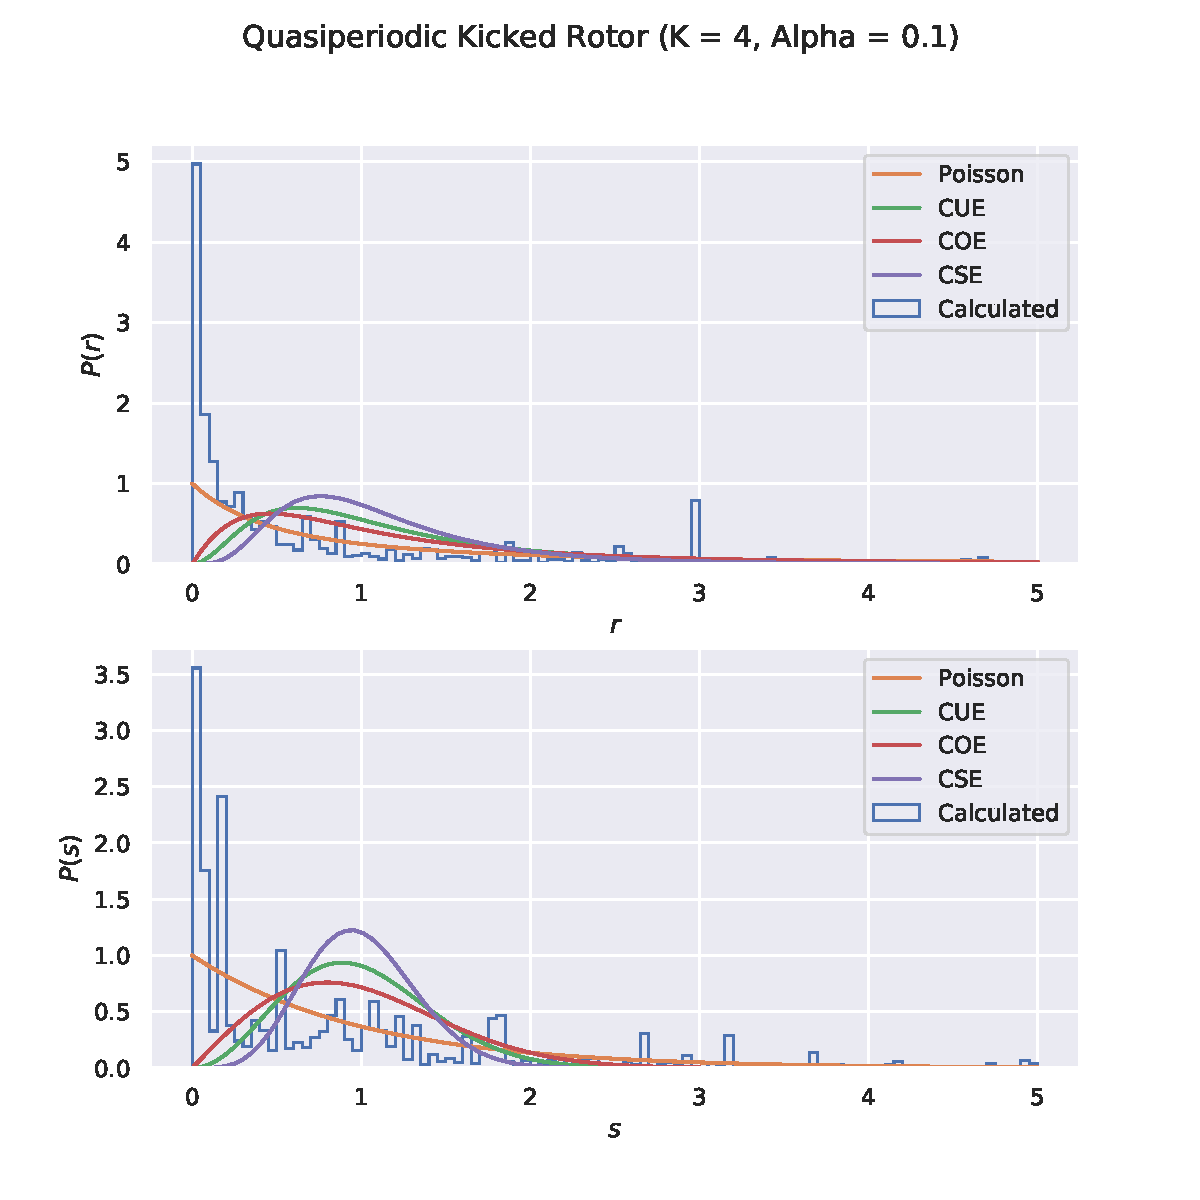
\includegraphics[width=\linewidth]{quasiperiodic_kickedrotor_spectrum_N10_precritical.pdf}
    \caption{Post-critical: $p$ in (-10, 10), K = 7, $\hbar$ = 2.85, $\alpha$ = 0.8,
    $\omega_2$ = $2\pi\sqrt{5}$, $\omega_3$ = $2\pi\sqrt{13}$, eigenphases
    used = 6934 and 2327 were discarded due to magnitude errors. $det(F) = 0$.}
    \centering
\end{figure}

\begin{figure}
    \centering
    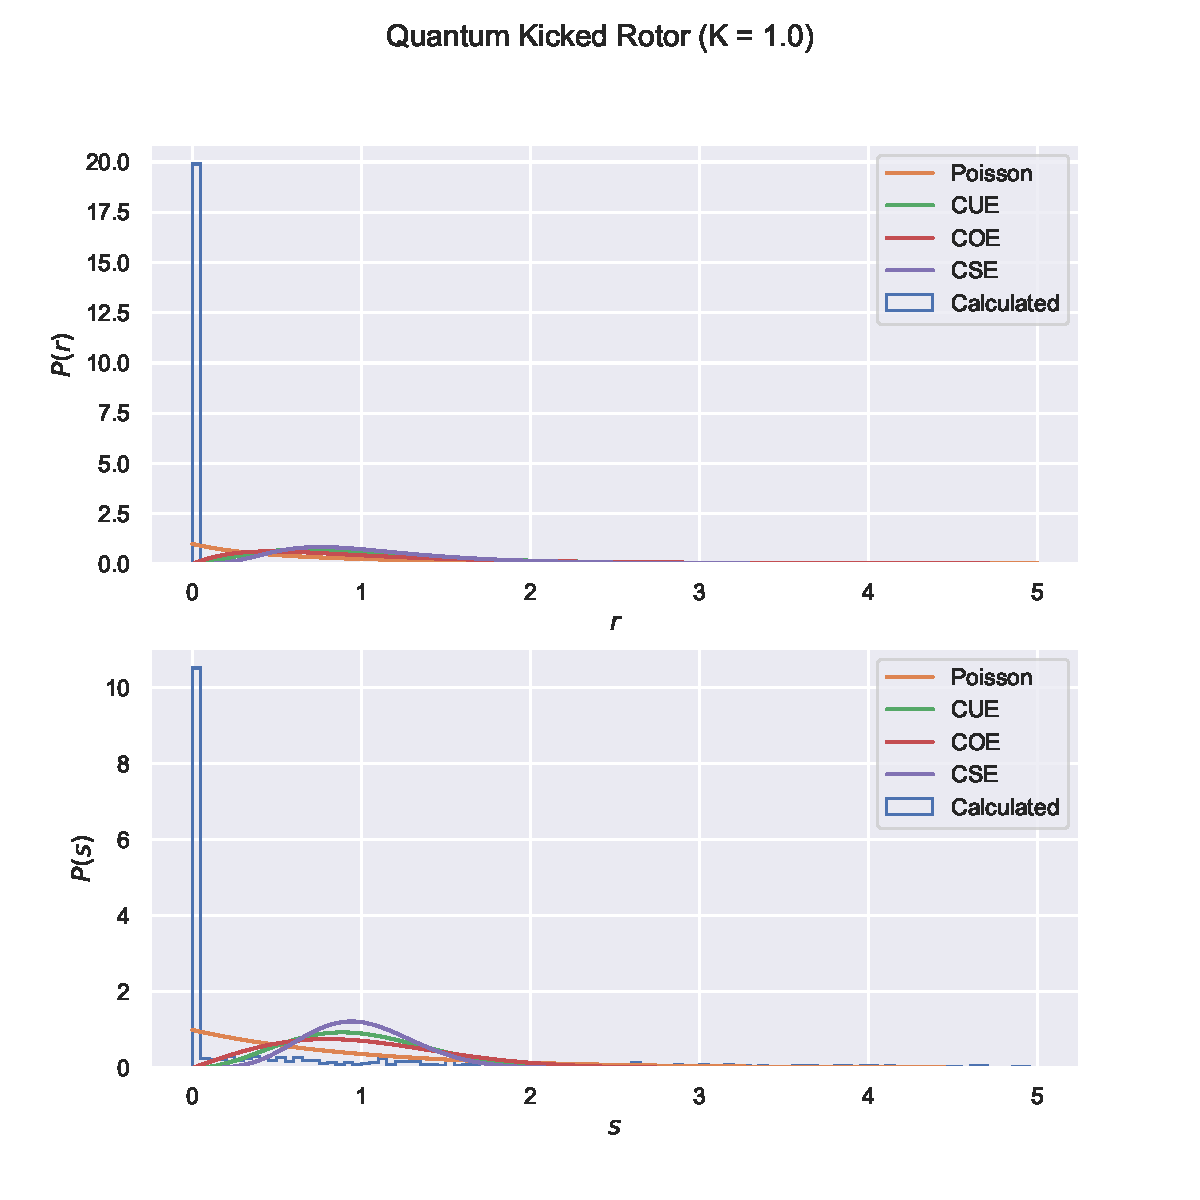
\includegraphics[width=\linewidth]{kickedrotor_spectrum_K1.0.pdf}
\end{figure}

\begin{figure}
    \centering
    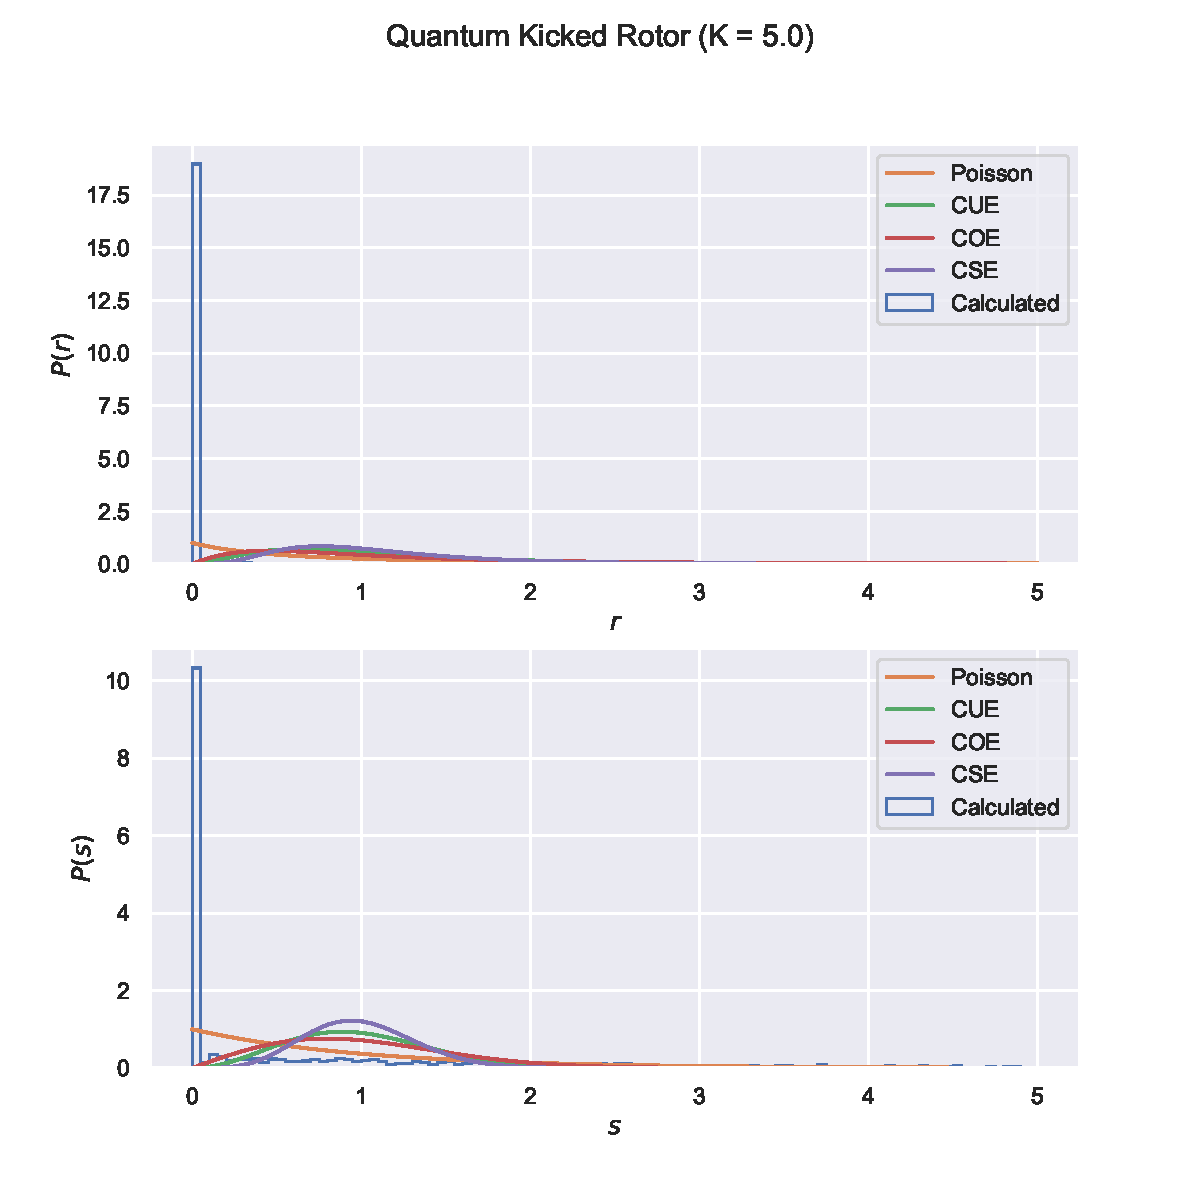
\includegraphics[width=\linewidth]{kickedrotor_spectrum_K5.0.pdf}
\end{figure}
\begin{figure}
    \centering
    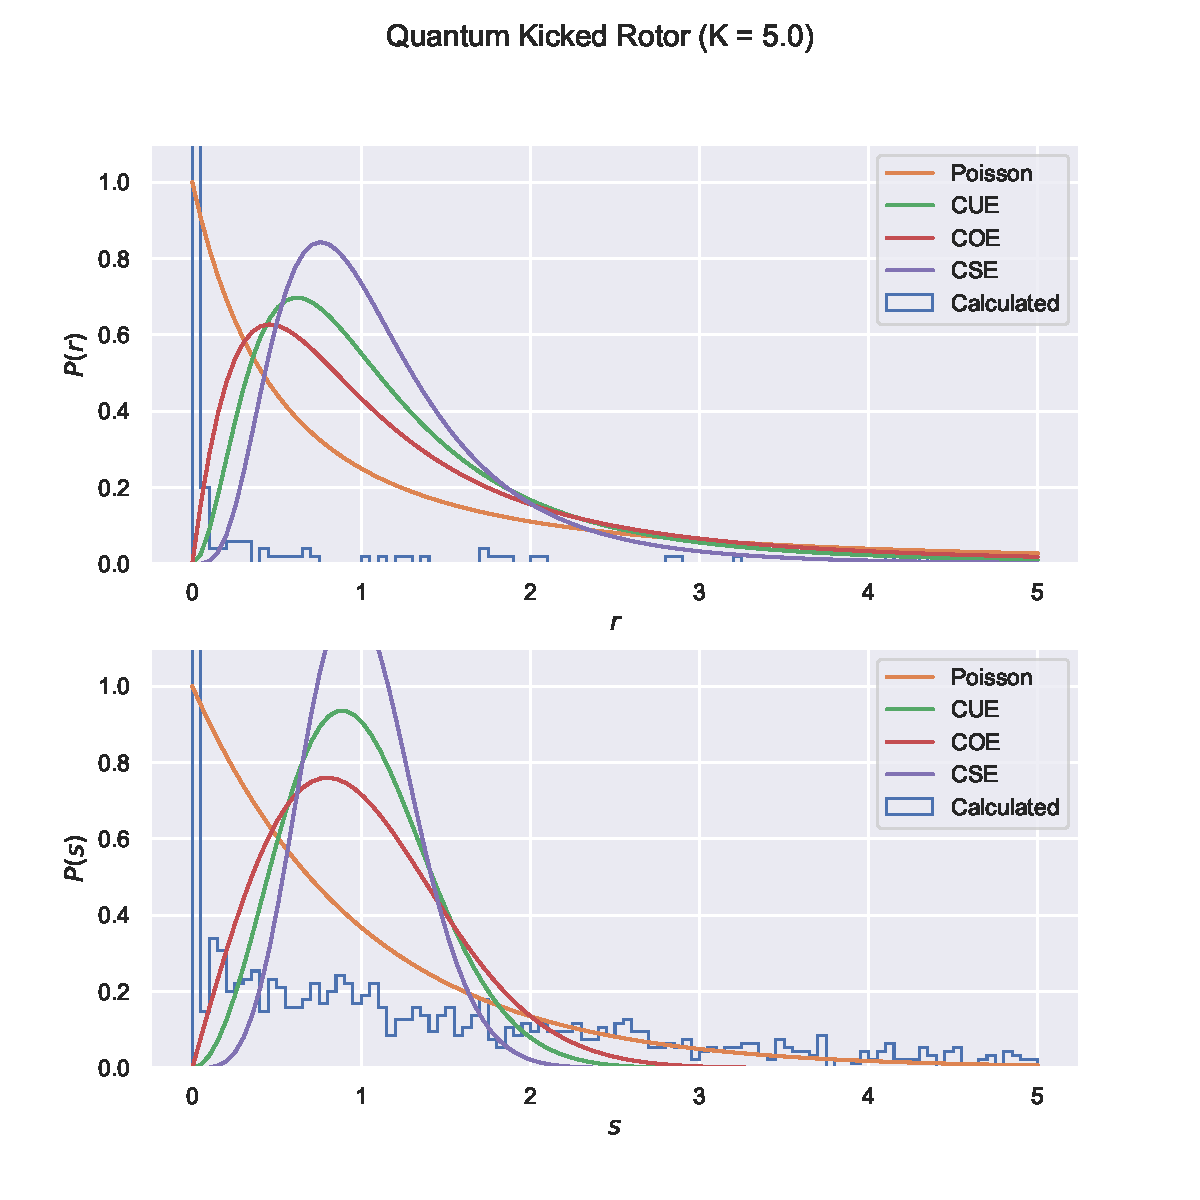
\includegraphics[width=\linewidth]{kickedrotor_spectrum_K5.0_magnified.pdf}
\end{figure}
\begin{figure}
    \centering
    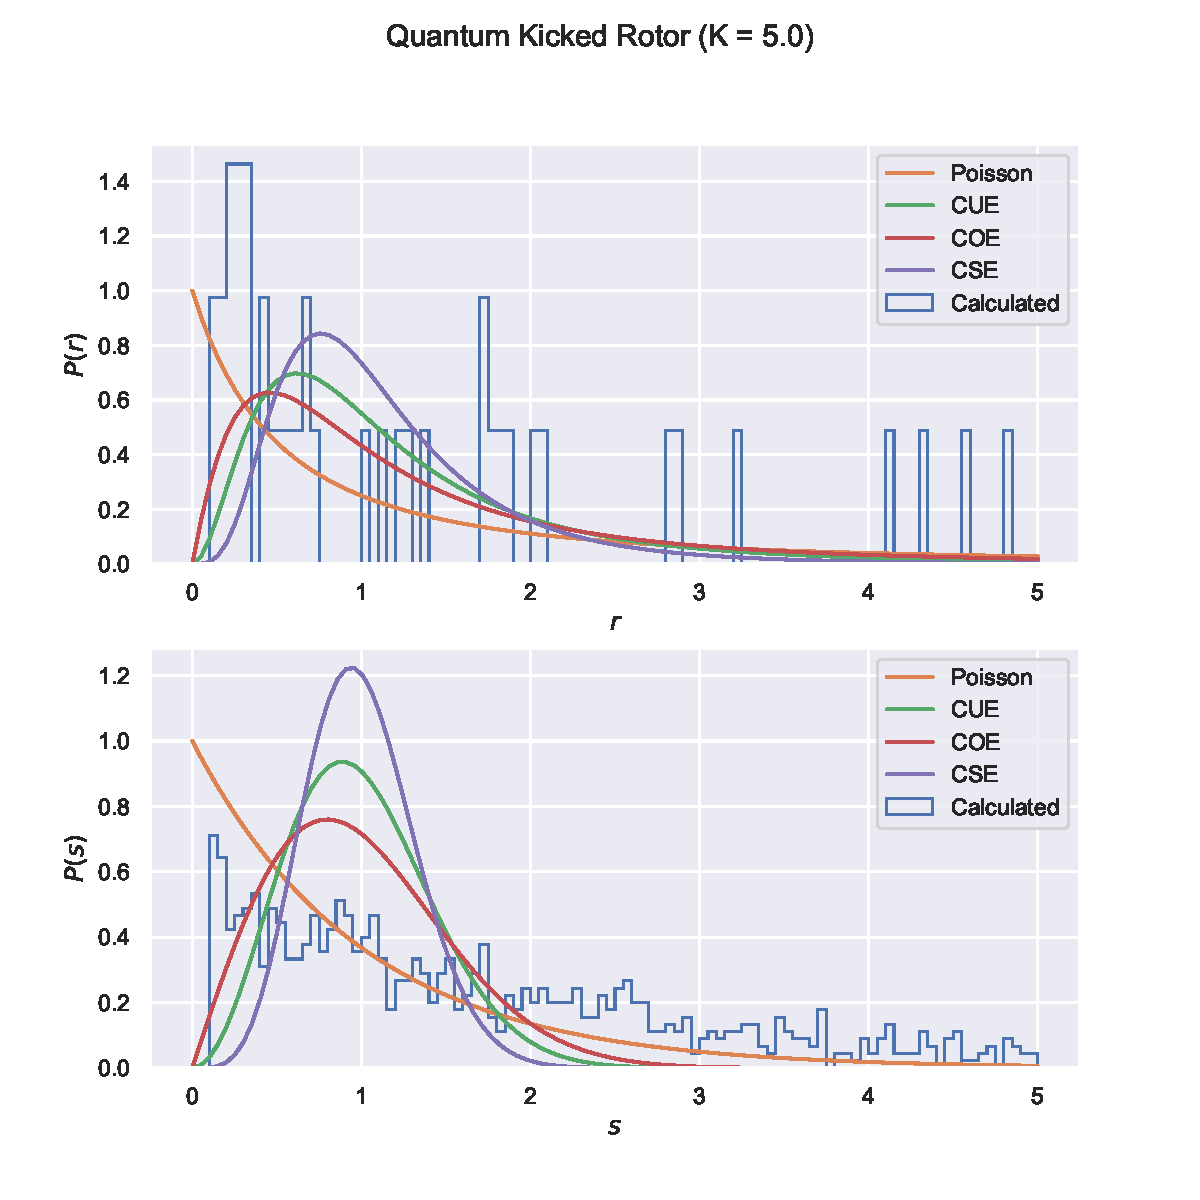
\includegraphics[width=\linewidth]{kickedrotor_spectrum_K5.0_suppressed.pdf}
\end{figure}
\begin{figure}
    \centering
    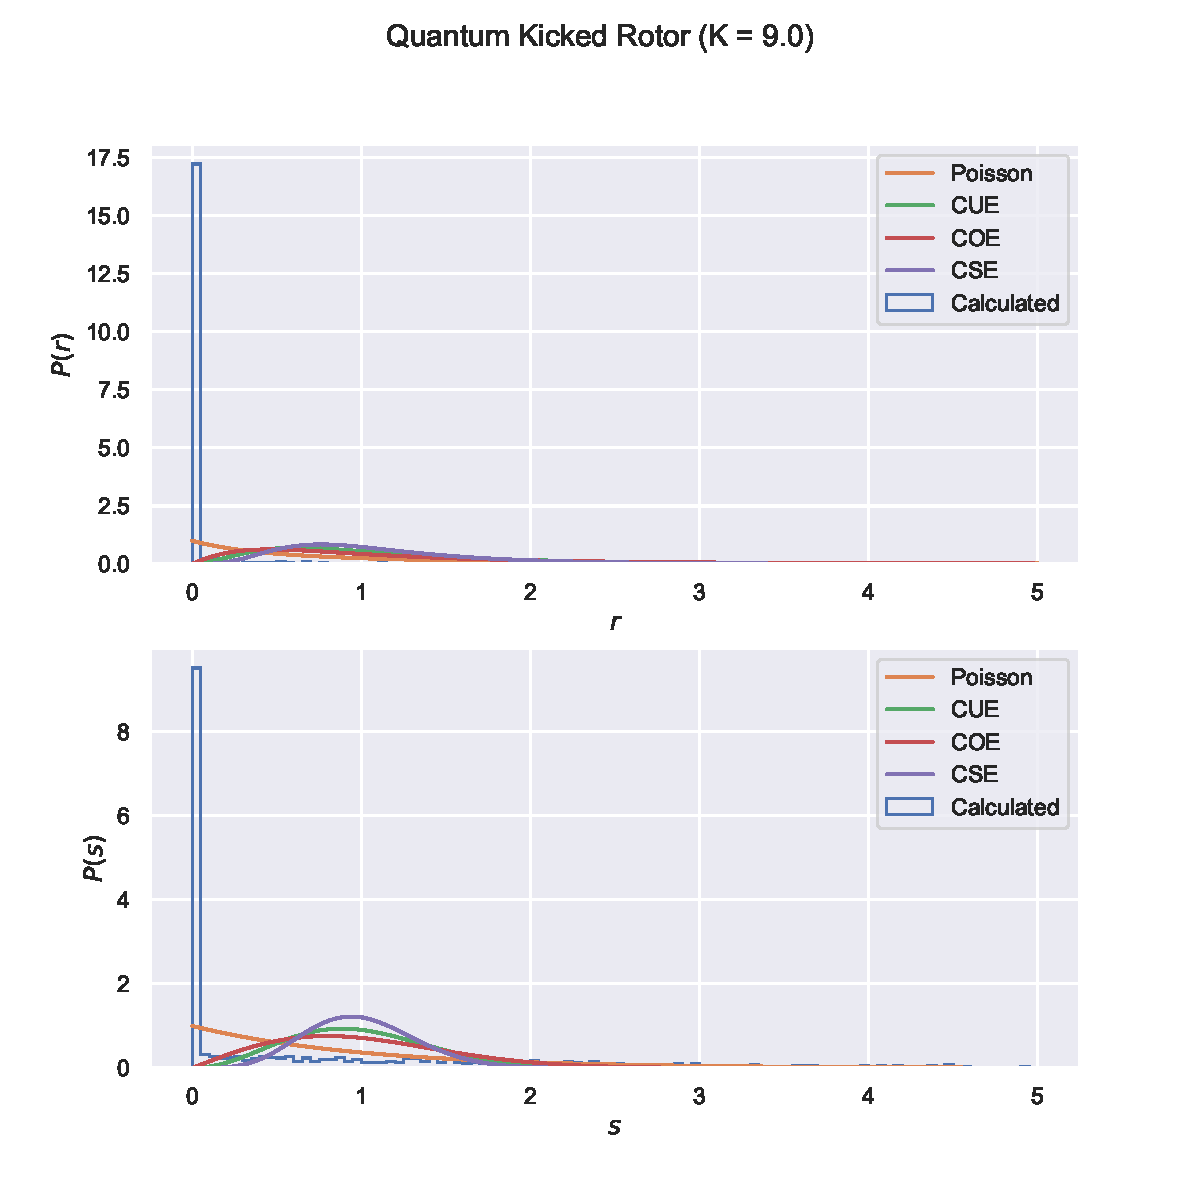
\includegraphics[width=\linewidth]{kickedrotor_spectrum_K9.0.pdf}
\end{figure}
\begin{figure}
    \centering
    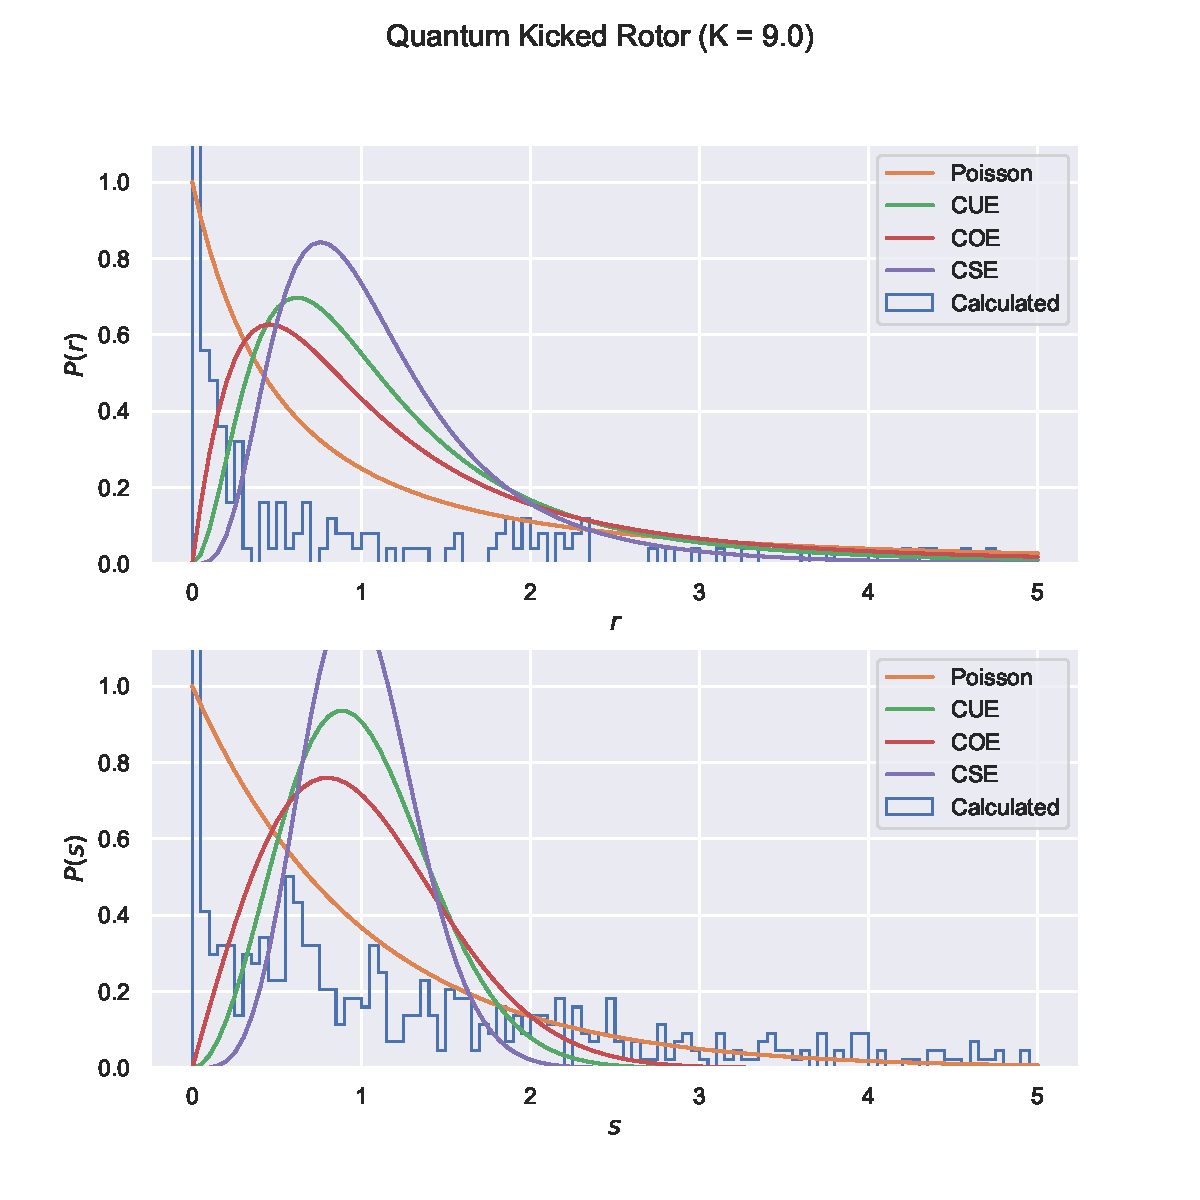
\includegraphics[width=\linewidth]{kickedrotor_spectrum_K9.0_magnified.pdf}
\end{figure}
\begin{figure}
    \centering
    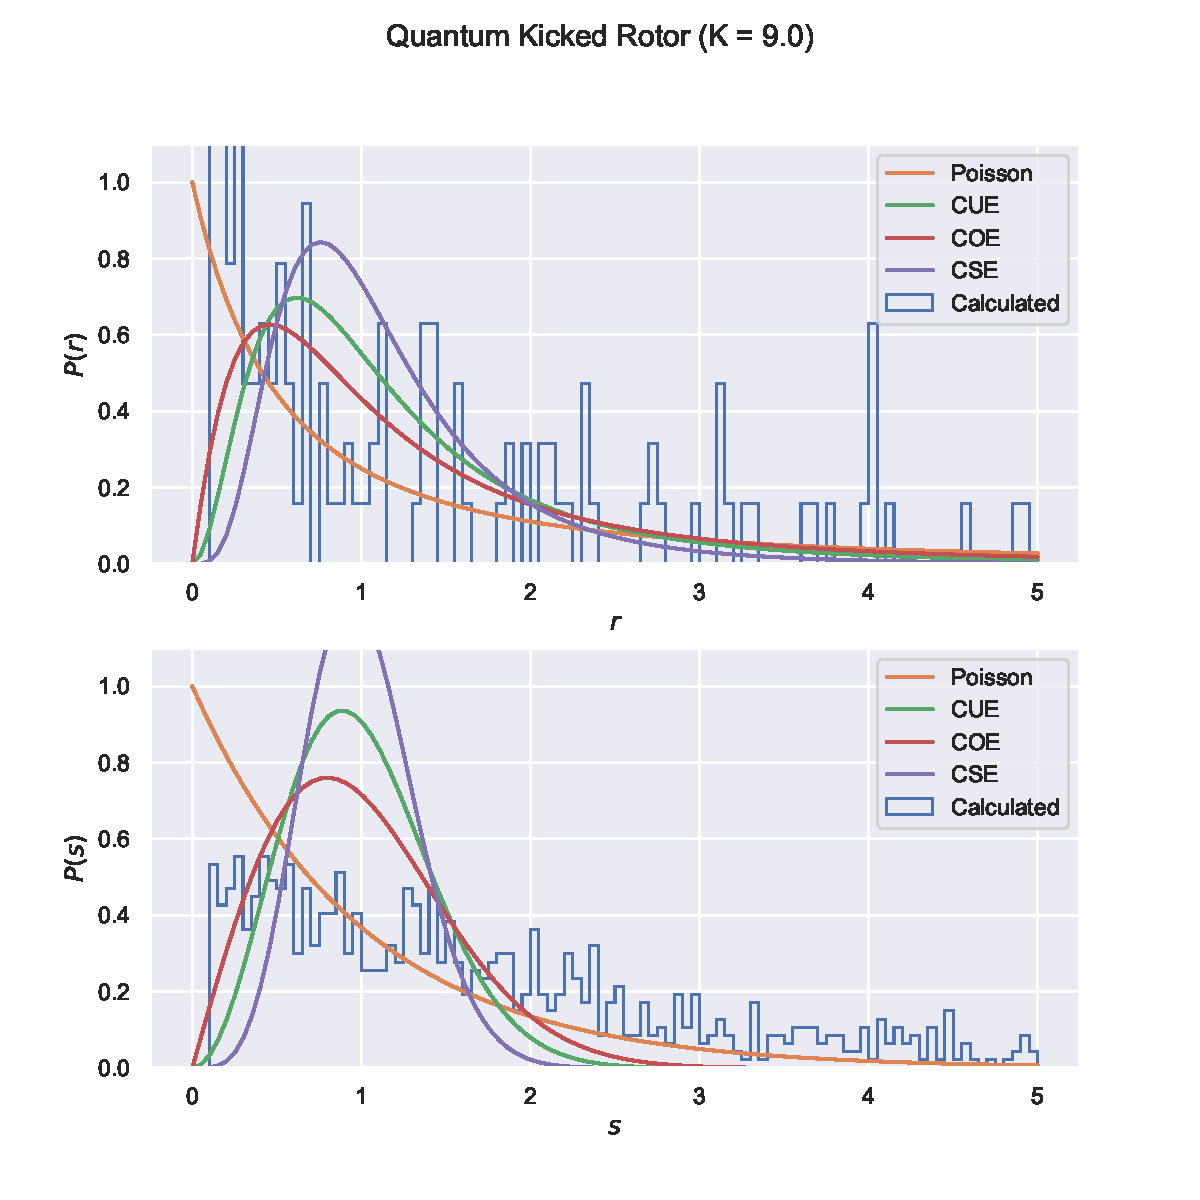
\includegraphics[width=\linewidth]{kickedrotor_spectrum_K9.0_magnified_suppressed.pdf}
\end{figure}

\newpage
\section{June 20, 2021}

\begin{equation}
    H = \frac{P^2}{2} + K cos(\theta) \sum_{n} \delta (t - n\tau)
\end{equation}

This $H$ is symmetric under time reversal (if we consider only $t = n\tau$).
It is not rotationally invariant but it has spin 0, therefore, it falls in the
orthogonal symmetry class. But the Hamiltonian also has parity symmetry:
$\theta \to -\theta$, $P \to -P$. And so does the floquet operator. So we have
$[\Pi, F] = 0$. This complicates matters for us as the spectral statistics
needs to happen on the same quantum numbers. So we need to find a way to obtain
eigenvalues of only even or only odd eigenstates of $F$. There are issues with
this as the eigenvalue convergence is better than the eigenvector
convergence. For $DIM = 2001$ etc, the eigenvectors found are not so accurate
that we can be sure that they are either even or odd. Most of them are neither.

\nocite{*}
\printbibliography

\end{document}
